\documentclass[a4paper,11pt]{article}
\usepackage[russian]{babel} 
\usepackage[utf8x]{inputenc}
\usepackage{graphicx}
\usepackage[top=2cm,bottom=1.5cm,left=1cm,right=1cm]{geometry}
\usepackage{enumitem}
 \usepackage[warn]{mathtext} 

\begin{document}
 	\begin{center}
 		\begin{Large}
 			Домашняя работа №1
 		\end{Large}
 		\\
 		\medskip
 			"\textbf{Вычисление центра тяжести плоской фигуры}"
 			\\
			\medskip
			Вариант 6
 	\end{center}
 	\begin{flushleft}
	\textbf{\textit{Задание :}}
	\\ 	
 	\hangindent=1.5cm \hangafter=0 \noindent
 		Найти центр тяжести плоской фигуры, указанной на рисунке 1.
 	\end{flushleft} 	
 	\begin{figure}[h]
		\begin{center}
			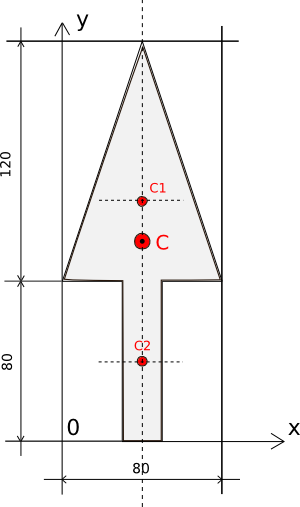
\includegraphics[scale=0.8]{images/final_draw.png}
			\caption{}			
		\end{center}
		\label{model}		
	\end{figure}
 	\begin{flushleft}
	\textbf{\textit{Решение :}}
	\\ 	
 	\hangindent=1cm \hangafter=0 \noindent
 		Для нахождения центра тяжести данной фигуры воспользуемся методом разбиения.	\\
 		Данная фигура состоит из 2 фигур:
 		\begin{enumerate}
 			\item Треугольника с вершинами, условно обозначенными как $(x_1,y_1)$, $(x_2,y_2)$, $(x_3,y_3)$
 			\item Треугольника с вершинами, условно обозначенными как $(x_1,y_1)$, $(x_2,y_2)$, $(x_3,y_3)$, $(x_4,y_4)$
 		\end{enumerate}
 		Введем декартову систему координат $O_{XY}$ с центром в точке $O (0,0)$.Отметим также что так как исходная плоская фигура симметрична, то и центр тяжести этой фигуры будет лежать на оси симметрии этой фигуры.  
 		\begin{enumerate}[label=\Roman{*}, ref=(\roman{*})]
 			\item Находим координаты точки центра тяжести треугольника, обозначив эту точку $C_1$.$C_1$ находится на пересечении медиан треугольника, а её координаты представляют собой среднее арифметическое суммы координат соответствующих вершин
 			\newpage
 			\begin{equation}
 				(C_1)_x = \frac{x_1+x_2+x_3}{3} = \frac{0+40+80}{3} = 40
 			\end{equation}
 			\begin{equation}
 				(C_1)_y = \frac{y_1+y_2+y_3}{3} = \frac{80+200+80}{3} = 120 
\end{equation}
 		Найдем также и площадь треугольника ${S_1}$ : ${S_1 = \frac{1}{2}\cdot(80\cdot120)} = 4800$. 
 		\item Найдем координаты точки центра тяжести ${C_2}$ прямоугольника, находящиеся на пересечении диагоналей :
 			\begin{equation}
 				(C_2)x = \frac{80}{2} = 40
			\end{equation}
			 \begin{equation}
 				(C_2)y = \frac{80}{2} = 40
			\end{equation}
			Площадь прямоугольника ${S_2}$ : ${S_2 = 80\cdot20=1600}$  							\item
			Зная координаты центров тяжести составных плоских фигур, а также их площади, можно найти координаты точки центра тяжести ${C}$ исходной плоской фигуры по формулами :
			\begin{equation}
				x_c = \frac{x_{c1}\cdot S_1 + x_{c2}\cdot S_2}{S_1 + S_2}
			\end{equation}
			\begin{equation}
				y_c = \frac{y_{c1}\cdot S_1 + y_{c2}\cdot S_2}{S_1 + S_2}
			\end{equation}
			Найдем координаты, подставив известные значения : 
			\begin{equation}
				x_c = \frac{40\cdot 4800 + 120\cdot 1600}{4800 + 1600} = 40
			\end{equation}
			\begin{equation}
				y_c = \frac{40\cdot 4800 + 40\cdot 1600}{4800 + 1600} = 100
			\end{equation}
					Центром тяжести плоской фигуры, изображённой на рисунке на 1, является точка   
$C$ с координатами $(40,120)$.			  
 		\end{enumerate}
	
 	\end{flushleft} 		
\end{document} 	 	

 
